\documentclass[a4paper,12pt]{article} 
\usepackage[T2A]{fontenc}			
\usepackage[utf8]{inputenc}			
\usepackage[english,russian]{babel}	
\usepackage{amsmath,amsfonts,amssymb,amsthm,mathrsfs,mathtools} 
\usepackage{cancel}
\usepackage{hhline}
\usepackage{multirow}
\usepackage[colorlinks, linkcolor = purple, citecolor = purple]{hyperref}
\usepackage{upgreek}\usepackage[left=2cm,right=2cm,top=2cm,bottom=3cm,bindingoffset=0cm]{geometry}
\usepackage{tikz}
\usepackage{graphicx}
\usepackage{subfig}
\usepackage{titletoc}
\usepackage{pgfplots}
\usepackage{xcolor}
\usepackage{wrapfig}

\newcommand{\angstrom}{\text{\normalfont\AA}}
\author{Дорогинин Д.В.\\
Группа Б02-825}
\title{5.1.3. Эффект Рамзауэра.}
\date{}

%\begin{wrapfigure}{r}{0.5\textwidth}
%\begin{center}
%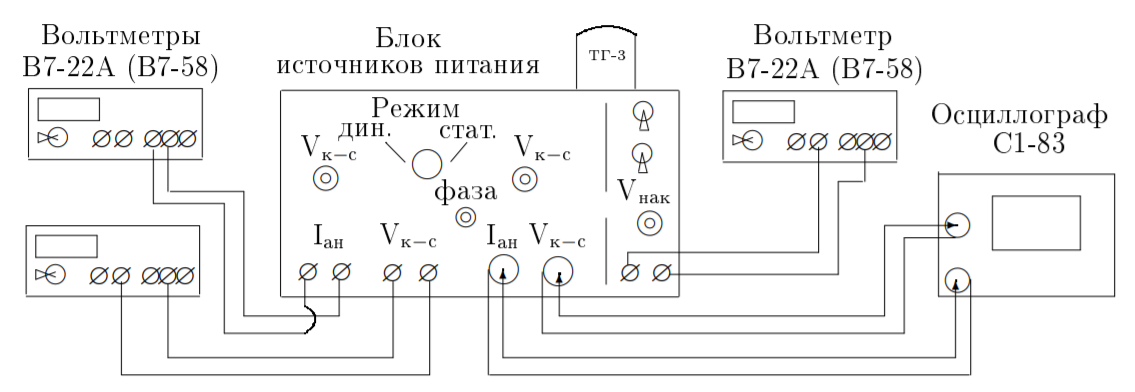
\includegraphics[width = 0.4\textwidth]{1.png}
%\end{center}
%\caption{}
%\end{wrapfigure}

%\begin{wrapfigure}{r}{0.5\textwidth}
%\begin{center}
%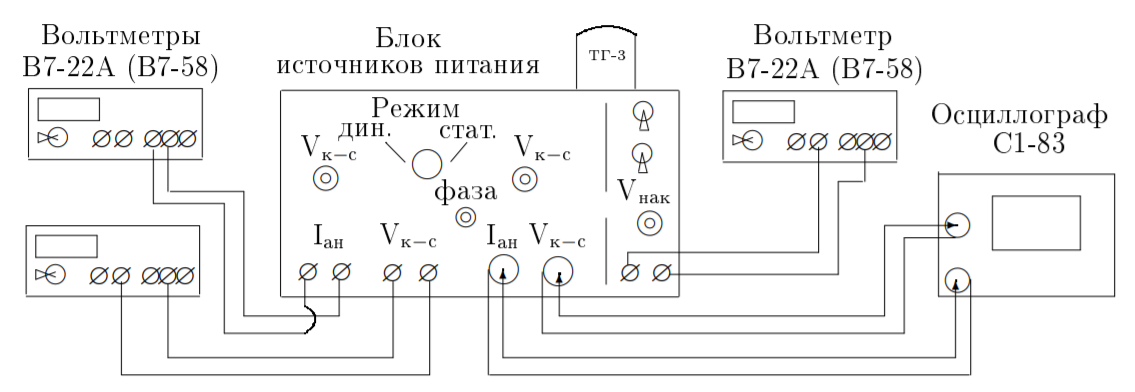
\includegraphics[width = 0.4\textwidth]{1.png}
%\end{center}
%\caption{}
%\end{wrapfigure}

\begin{document}
\maketitle
\textbf{В работе}: исследуется энергетическая зависимость вероятности рассеяния электронов атомами инертного газа, определяются энергии электронов при которых наблюдается <<просветление>> инертного газа и оценивается размер его внешней электронной оболочки.

\section*{Теория}
Рассеяние электрона на атоме можно приближённого рассматривать как рассеяние частицы энергии $E$ на потенциальной яме длины $\ell$ и глубины $U_0$. Уравнение Шрёдингера имеет вид
\[\Psi'' + k^2 \Psi = 0,\]
где вне ямы 
\[k^2 = k_1^2 = \dfrac{2mE}{\hbar^2},\]
а внутри 
\[k^2 = k_2^2 = \dfrac{2m(E+U_0)}{\hbar^2}.\]
Коэффициент прохождения в таком случае равен
\[D = \dfrac{16 k_1^2 k_2^2}{16k_1^2 k_2^2 + 4(k_1^2 - k_2^2)^2\sin^2(k_2\ell)}.\]
Заметим, что коэффициент прохождения имеет ряд максимумов и минимумов. Он максимальнем при
\begin{equation}\label{0}
\sqrt{\dfrac{2m(E+U_0)}{\hbar^2}}\ell = n\pi,~n=1,2,3,\dots
\end{equation}

Качественно эффект Рамзауэра можно объяснить, рассмотрев интерференцию прошедшей и дважды отразившейся от оболочки волн де Бройля. Длины волн вне и внутри атома:
\[\lambda = \dfrac{h}{\sqrt{2mE}},~\lambda_1 = \dfrac{h}{\sqrt{2m(E+U_0)}}.\]
Соответственно условия на первые интерфереционные максимум и минимум 
\begin{equation}\label{1}
2\ell = \dfrac{h}{\sqrt{2m(E_1 + U_0)}},~2\ell = \dfrac{3}{2}\dfrac{h}{\sqrt{2m(E_2 + U_0)}}.
\end{equation}
Исключая из этих соотношений глубину ямы, получим
\begin{equation}\label{2}
\ell = \dfrac{h\sqrt{5}}{\sqrt{32m(E_2 - E_1)}}.
\end{equation}
Глубина ямы при этом равна
\begin{equation}\label{4}
U_0 = \dfrac{4}{5}E_2 - \dfrac{9}{5}E_1.
\end{equation}
\section*{Описание установки}
\begin{figure}[h]
    \subfloat{{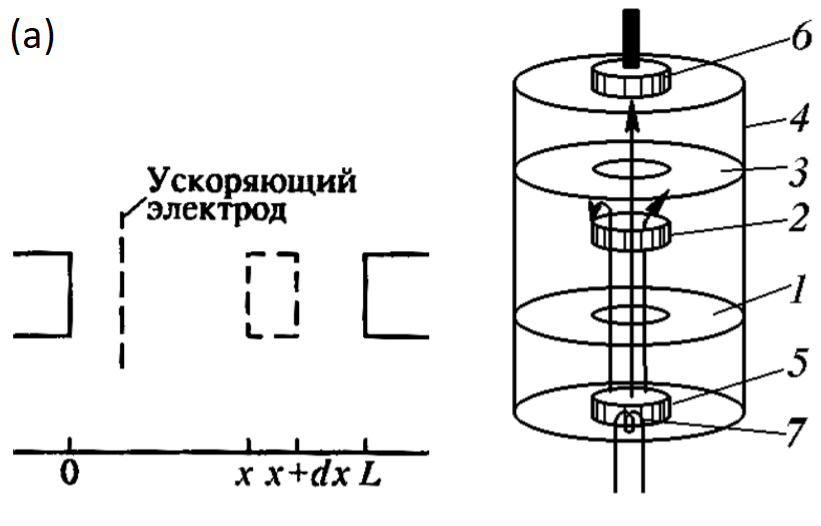
\includegraphics[width=0.42\textwidth]{2.png}}}
    \subfloat{{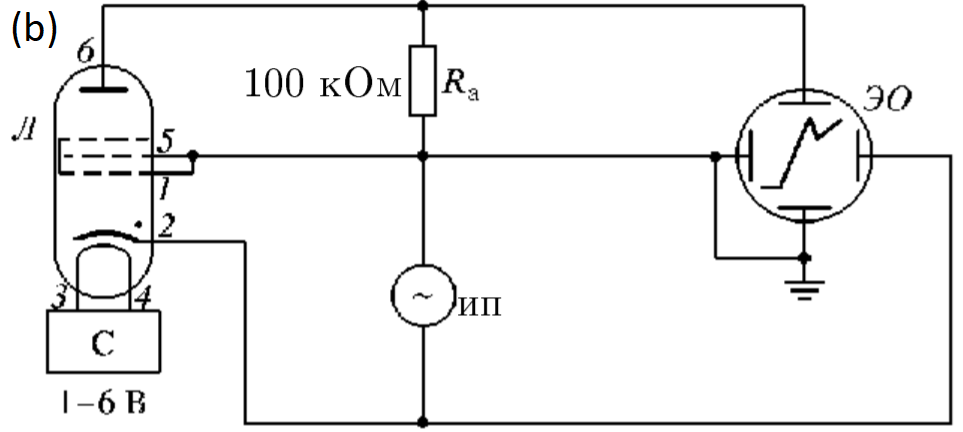
\includegraphics[width=0.58\textwidth]{3.png}}}
  \centering
  \caption{(a) Схема тиратрона (слева) и его конструкция (справа): 1,2,3 -- сетки, 4 -- внешний металлический цилиндр, 5 -- катод, 6 -- анод, 7 -- накаливаемая спираль. (b) Схема включения тиратрона.}
\end{figure}
Для изучения эффекта испульзуется тиратрон ТГ3-01/1.3Б, заполненный инертным газом (Рис. 1а). Электроны эмитируются катодом, ускоряются напряжением $V$ и рассеиваются на атомах газа. Сетки соединены между собой и имеют один потенциал, примерно равный потенциалу анода. Рассеянные электроны отклоняются и уходят на сетку, а оставшиеся достигают анода, создавая ток $I_\text{a}$. Таким образом, поток электронов на расстоянии $x$ от ускоряющей сетки уменьшается с ростом $x$. ВАХ анода должна быть
\begin{equation}\label{3}
I_\text{a} = I_0 \exp\left( - C w(V) \right),
\end{equation}
где $I_0 = eN_0$ -- ток катода, $I_\text{a} = eN_a$ -- ток анода, $C = Ln_\text{a} \Delta_\text{a}$($L$ --  расстояние между катодом и анодом, $\Delta_\text{a}$ -- площадь поперечного сечения атома, $n_\text{a}$ -- концентрация газа в лампе), $w(V)$ -- вероятность рассеяния на атоме.
Формулу \eqref{3} можно переписать в виде
\[\tag{5a}\label{5a}
w(V) = -\dfrac{1}{C}\ln \dfrac{I_\text{a}(V)}{I_0}.
\]
\begin{figure}[h]
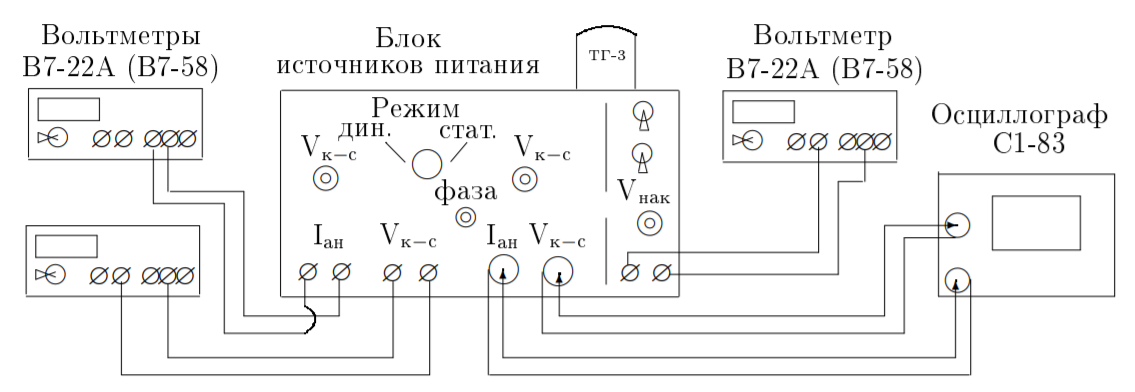
\includegraphics[scale=0.6]{1.png}
\centering
\caption{Схема установки.}
\end{figure}\\
Схема экспериментальной установки, изображанная на Рис. 1b, в нашей работе конструктивно осуществлена следующим образом (Рис. 2): лампа-тиратрон расположена непосредственно на корпусе блока источников питания (БИП), напряжение к электродам лампы подаётся от источников питания, находящихся в корпусе прибора. Регулировка напряжения и выбор режима работы установки производится при помощи ручек управления, выведенных на лицевую панель БИП.
\section*{Ход работы и обработка данных}
С помощью осциллографа снимаем ВАХ в динамическом режиме при двух различных напряжениях накала, погрешность их измерения берём $\sigma_U = 0.01~\text{В}$, так как регистрируемое вольтметром значение не было постоянным, а колебалось в последнем знаке. По ВАХ определим $V_{\text{max}}$, $V_{\text{min}}$ и $V_{\text{пробой}}$ (Таблица 1). Погрешности всех измерений с осциллографе -- $\sigma_V = 0.3~\text{В}$ -- цена деления, умноженная на $\sqrt{2}$, так как точки на двух кривых неточно совпадали по своему положению.
\begin{figure}[h]
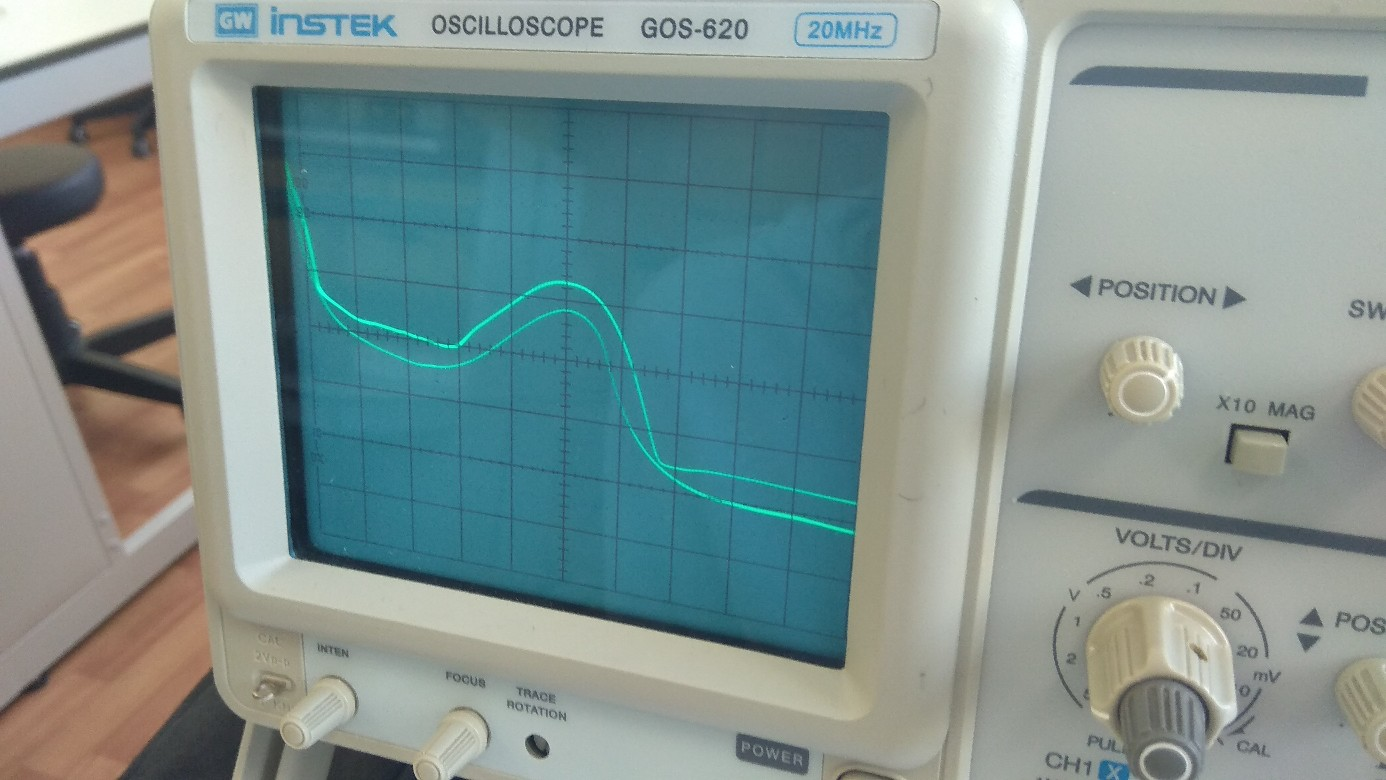
\includegraphics[width=0.6\textwidth]{4.jpg}
\centering
\caption{ВАХ, наблюдаемая на осциллографе ($V = 2.67~\text{В}$).}
\end{figure}
\begin{table}[h]
\begin{tabular}{|c|c|c|c|c|c|c|}
\hline
  & $U$, В & $\sigma_U$, В & $V_{\text{max}}$, В & $V_{\text{min}}$, В & $V_{\text{пробой}}$, В & $\sigma_V$, В \\ \hline
1 & 2.67   & 0.01          & 3.0                   & 7.4                 & 11.4                   & 0.3           \\ \hline
2 & 2.96   & 0.01          & 2.0                   & 7.4                 & 11.2                   & 0.3           \\ \hline
\end{tabular}
\centering
\caption{Измерения по ВАХ.}
\end{table}\\
Рассчёт $\ell$ по формулам \eqref{1} неточен, так как яма меньше предполагаемых $U_0 = 2.5~\text{эВ}$. Поэтому найдём $\ell$ и глубину ямы по формулам \eqref{2} и \eqref{4} (результат -- среднее по двум опытам):
\[\ell = 4.4 \pm 0.4~\angstrom,\]
\[U_0 = 0.7 \pm 0.2~\text{эВ}.\]
Все погрешности посчитаны по стандартным формулам погрешности сложной величины, то есть корень суммы произведений квадратов частных производных по величине на квадрат её погрешности. Оценим ионизационный потенциал как 
\[U = U_0 + V_{\text{пробой}} = 12.0 \pm 0.4~\text{эВ}.\]
Сравнивая с потенциалами ионизации, приведёнными в \cite{laba} (описание работы 1.3), видим, что полученный потенциал в пределах погрешности совпадает с ионизационным потенциалом ксенона $U = 12.1~\text{эВ}$.\\
Теперь снимем ВАХ титратрона в статическом режиме при тех же значениях напряжения накала, данные представлены в Таблице 3 (погрешности -- последний знак, показываемый вольтметром, максимумы и минимумы выделены, их погрешности -- минимум расстояния до соседней точки), а графики -- на Рис. 4. Проведя аналогичные расчёты, получим:
\[\ell = 2.62\pm 0.02~\angstrom,\]
\[U_0 = 1.35\pm 0.03~\text{эВ}.\]
Из формулы \eqref{0} оценим значения напряжений максимумов порядка $n > 2$:
\[E_2 = 20.41~\text{эВ},~E_2 = 47.61~\text{эВ},~E_4 = 85.69~\text{эВ}.\]
Полученные энергии выше потенциала ионизации, поэтому эти максимумы уже не будут наблюдаться.
\begin{figure}[h]
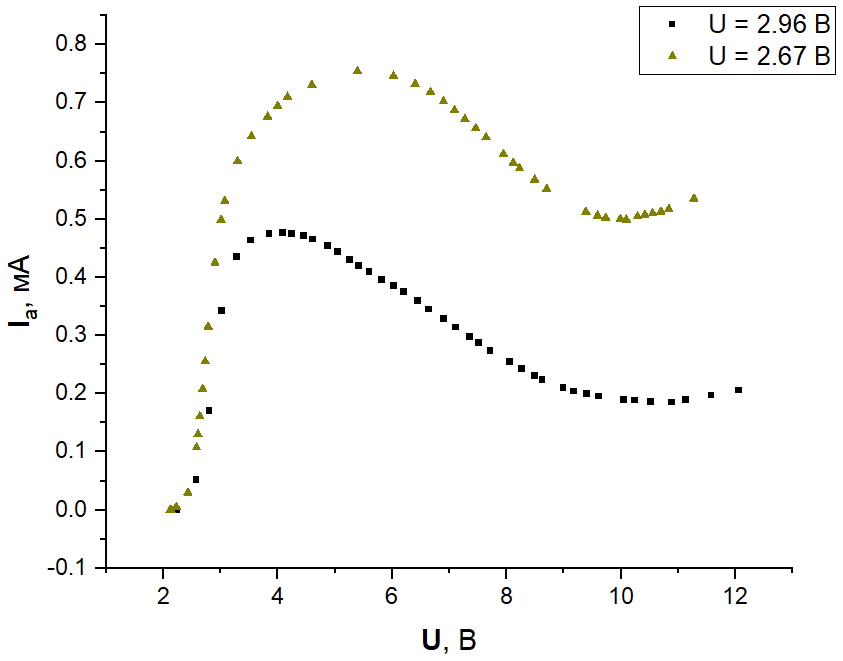
\includegraphics[width=0.7\textwidth]{4.png}
\centering
\caption{ВАХ титратрона при разных напряжениях накала.}
\end{figure}\\
Наконец, в соответствии с \eqref{5a}, можно получит зависимость вероятности рассеяния от напряжения на титротроне. Качественный график приведён на Рис. 5. 
\begin{figure}
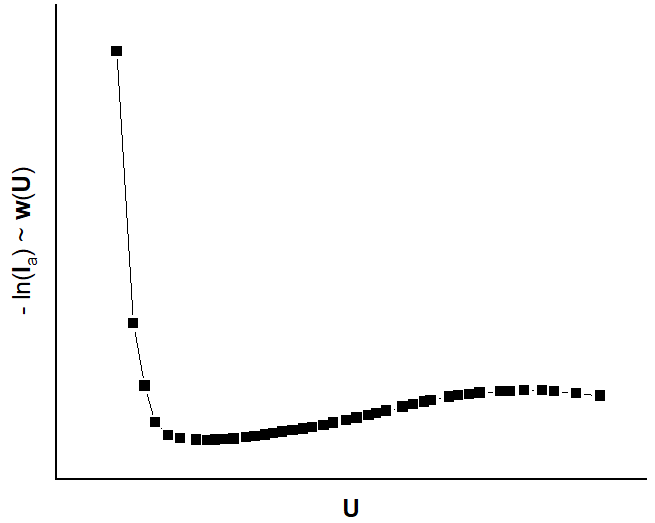
\includegraphics[width = 0.7\textwidth]{5.png}
\centering
\caption{Качественный вид зависимости $w = w(V)$.}
\end{figure}



\begin{table}[h]
\begin{tabular}{|c|c|c|c|c|c|c|c|c|c|c|c|}
\hline
                 & \multicolumn{11}{c|}{$U_\text{накала} =   2.67~\text{В}$}                             \\ \hline
$U$, В           & 2.12  & 2.14  & 2.23  & 2.43  & 2.58  & 2.61  & 2.64  & 2.69  & 2.73  & 2.78  & 2.90  \\ 
$I_\text{a}$, мА & 0.000 & 0.000 & 0.006 & 0.030 & 0.108 & 0.130 & 0.161 & 0.208 & 0.256 & 0.315 & 0.426 \\ \hline
$U$, В           & 3.01  & 3.08  & 3.30  & 3.54  & 3.82  & 4.00  & 4.17  & 4.59  & \textbf{5.39}  & 6.02  & 6.40  \\ 
$I_\text{a}$, мА & 0.499 & 0.532 & 0.600 & 0.642 & 0.676 & 0.695 & 0.710 & 0.731 & \textbf{0.755} & 0.746 & 0.732 \\ \hline
$U$, В           & 6.67  & 6.90  & 7.09  & 7.27  & 7.46  & 7.64  & 7.94  & 8.12  & 8.23  & 8.49  & 8.70  \\ 
$I_\text{a}$, мА & 0.719 & 0.702 & 0.687 & 0.672 & 0.656 & 0.641 & 0.612 & 0.597 & 0.587 & 0.568 & 0.552 \\ \hline
$U$, В           & 9.39  & 9.59  & 9.73  & 9.99  & \textbf{10.09} & 10.29 & 10.42 & 10.55 & 10.70 & 10.84 & 11.27 \\ 
$I_\text{a}$, мА & 0.513 & 0.506 & 0.503 & 0.500 & \textbf{0.499} & 0.505 & 0.508 & 0.511 & 0.513 & 0.517 & 0.536 \\ \hline
                 & \multicolumn{11}{c|}{$U_\text{накала} =   2.96~\text{В}$}                             \\ \hline
$U$, В           & 2.24  & 2.58  & 2.81  & 3.02  & 3.29  & 3.53  & 3.85  & \textbf{4.09}  & 4.25  & 4.46  & 4.61  \\ 
$I_\text{a}$, мА & 0.000 & 0.052 & 0.171 & 0.342 & 0.435 & 0.464 & 0.475 & \textbf{0.476} & 0.476 & 0.471 & 0.466 \\ \hline
$U$, В           & 4.87  & 5.04  & 5.26  & 5.42  & 5.60  & 5.82  & 6.03  & 6.21  & 6.45  & 6.64  & 6.91  \\ 
$I_\text{a}$, мА & 0.454 & 0.444 & 0.431 & 0.420 & 0.409 & 0.396 & 0.385 & 0.375 & 0.359 & 0.345 & 0.328 \\ \hline
$U$, В           & 7.12  & 7.36  & 7.51  & 7.72  & 8.05  & 8.26  & 8.49  & 8.62  & 8.99  & 9.18  & 9.40  \\ 
$I_\text{a}$, мА & 0.314 & 0.298 & 0.288 & 0.274 & 0.255 & 0.243 & 0.231 & 0.224 & 0.210 & 0.204 & 0.200 \\ \hline
$U$, В           & 9.62  & 10.04 & 10.24 & 10.52 & \textbf{10.89} & 11.13 & 11.58 & 12.06 &       &       &       \\ 
$I_\text{a}$, мА & 0.195 & 0.189 & 0.189 & 0.186 & \textbf{0.185} & 0.189 & 0.198 & 0.206 &       &       &       \\ \hline
\end{tabular}
\centering
\caption{Измерения для ВАХ титратрона.}
\end{table}
\section*{Заключение}
В ходе работы была статическим и динамическим методом исследована ВАХ титратрона, в обоих случаях соответствующая теоретической, получено значение размера внешней оболочки атома инертного газа и потенциал его ионизации, по которому было определено, что это ксенон.
\begin{thebibliography}{9}
\bibitem{laba} 
Игошин Ф.Ф., Самарский Ю.А., Ципенюк Ю.М. 
\textit{Лабораторный практикум по общей физике: Учеб. пособие для вузов. Т. 3 Квантовая физика}. 
М.: Физматкнига, 2005.
\end{thebibliography}
\end{document}